\documentclass[../report_polarFIR.tex]{subfiles}
\begin{document}
\chapter{CORDIC}

The next unit in the processing chain, as shown in Figure \ref{processingChainGraph}, is the CORDIC rotational computer. The CORDIC is implemented in Vitis HLS using equations shown in section \ref{cordicTheory}. The CORDIC's inputs are specified on a range generated by the worst-case scenario of the FIR filter's behavior, which is $\pm 125000$ given an input to the FIR of $\pm 50$ (refer to section \ref{FIRdata}). Additionally the FIR filter outputs data in a cartesian $(x, y)$ form. The CORDIC recieves these vectors of the cartesian form 
\begin{equation}
	d = \alpha + j\beta
\end{equation}
and converts them into polar form
\begin{equation}
	d = (r, \theta)
\end{equation}
where
\begin{equation}
	r = \sqrt{a^2 + b^2}
\end{equation}
and
\begin{equation}
	\theta = \tan^{-1}\left({\frac{\beta}{\alpha}}\right)
\end{equation}

As discussed in section \ref{cordicTheory}, this calculation is not trivial. However, it is possible to translate the coordinate system shift into the algorithm seen below in Listing \ref{CORDICalgo}.

		\begin{singlespace}
            \lstinputlisting[breaklines=true,
            label={CORDICalgo},
            caption={CORDIC algorithm},
            style=c-style,
            language=C++,
            firstnumber=136,
            linerange={136-173},
            ]{../source/CORDIC.cpp}
        \end{singlespace}

Analysis of this algorithm shows that it is an iterative process that over/under rotates the vector at decrementing amounts until the target angle has been reached. The actual rotation of the vectors is accomplished via simple multiplication of a matrix, shown in equations \ref{CORDICxCalc} and \ref{CORDICyCalc}. 

One area not discussed in detail thus far is the range of input the CORDIC is able to take. The accelerator is only capable of operation in quadrants I and IV. Therefore, an initial coordinate shift may be necessary before the raw data is passed to the rotator algorithm itself. The specifics and details of this process are shown in Listing \ref{CORDICsource}.


\section{Performance of the CORDIC}

The performance of the CORDIC hinges on three main concepts. Precision, latency, and utilization. Latency and utilization carry the same nomenclature as the discussion in the FIR algorithm's performance (see section \ref{FIRperf}). Precision of the CORDIC is a separate metric from the other two, yet has substantial impact on those two parameters. The precision of the CORDIC algorithm is broadly dependent on the number of iterations the algorithm goes through to calculate the desired angle. As noted in section \ref{cordicTheory}, each subsequent iteration of the algorithm rotates the vector by a lesser amount, and as such we find for a given target angle $\Theta$, CORDIC-calculated angle $\theta$, and number of iterations $n$, 
\begin{equation}
	\Theta \approx lim_{n \rightarrow \infty} \theta
\end{equation}
is a valid approximation for the convergence of any given angle calculation.

A critical parameter of the convergence of the algorithm is the number of iterations, or rotations, to perform. A method to estimate the convergence of the CORDIC algorithm is to inspect the CORDIC gain coefficents calculated using equation \ref{gainEQ}. The inverse of these coefficients ($K_i ^{-1}$) can be plotted to show convergence of the coefficients, as shown in Figure \ref{CORDICcoeffPlot}.

\begin{figure}[h!]
\begin{center}
\label{CORDICcoeffPlot}
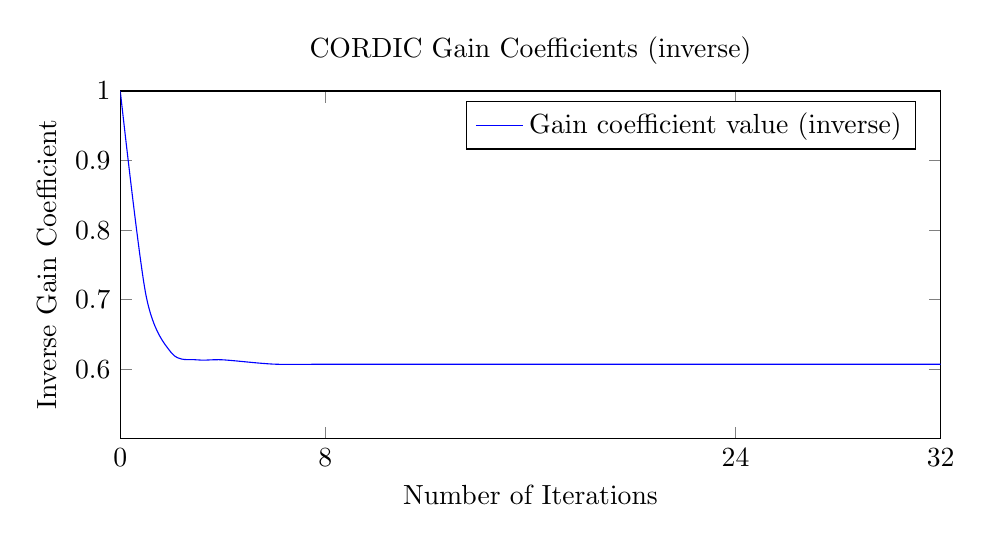
\begin{tikzpicture}

  \begin{axis}[    title={CORDIC Gain Coefficients (inverse)},    xlabel={Number of Iterations},    
         ylabel={Inverse Gain Coefficient},    
         xmin=0, 
         xmax=32,    
         ymin=0.5, 
         ymax=1,    
         xtick={0, 8, 24, 32, 40, 48, 56, 64},    
         ytick={0.6, 0.7,..., 1},   
         %ymode=lin, 
         legend pos=north east,    
         grid style={dashed,gray!50},    
         width=12cm, 
         height=6cm, 
     ]

\addplot[
color=blue,
mark=,
smooth,
]
coordinates {
(0,1)
(1,0.7071)
(2,0.6234)
(3,0.6135)
(4, 0.6135719910778963)
(6, 0.6073517701412959)
(8, 0.607259112298892)
(10, 0.6072530315291342)
(32, 0.6072529350088808)
};

\legend{Gain coefficient value (inverse)}

\end{axis}

\end{tikzpicture}

   
   \caption{Plot of CORDIC gain}
   
\end{center}

\end{figure}
\FloatBarrier

We observe a substantial convergence of the algorithm after approximately 8 iterations of the algorithm. The 8th iteration addresses rotations on the magnitude of $2^{-8}$, which is an extremely small rotation. Traditional \codeword{float} datatypes do not consider levels beyond this amount of percision, although it is important to preserve such precision as long as possible while performing rotations of a given vector. 

A similar pattern is observed with the rotational angle of a given increment. We construct a similar plot as shown below:


\begin{figure}[h!]
\begin{center}
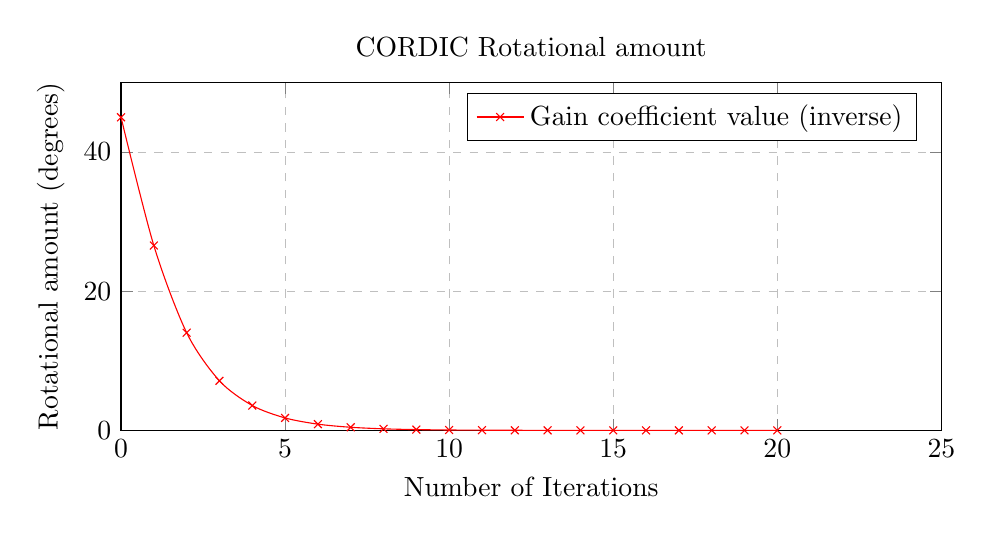
\begin{tikzpicture}

  \begin{axis}[    
  title={CORDIC Rotational amount},
      xlabel={Number of Iterations},
         ylabel={Rotational amount (degrees)},
         xmin=0,
         xmax=25,
         ymin=0,
         ymax=50,
         %ymode=log,
         xtick={0, 5,..., 25},    
         ytick={},    
         legend pos=north east,   
         xmajorgrids=true,
		 ymajorgrids=true,   
         grid style={dashed,gray!50},    
         width=12cm, 
         height=6cm,    ]
          
\addplot[
color=red,
mark=x,
smooth,
]
coordinates {
(0, 45)
(1, 26.565)
(2, 14.036)
(3, 7.125)
(4, 3.576)
(5, 1.790)
(6, 0.895)
(7, 0.4476)
(8, 0.2238)
(9, 0.1119)
(10, 0.0559)
(11, 0.0280)
(12, 0.0140)
(13, 0.0070)
(14, 0.0035)
(15, 0.0017)
(16, 0.0009)
(17, 0.0004)
(18, 0.0002)
(19, 0.0001)
(20, 0.0001)
};

\legend{Gain coefficient value (inverse)}

\end{axis}

\end{tikzpicture}

   
   \caption{Plot of CORDIC rotation per iteration}
   
\end{center}

\end{figure}
\FloatBarrier


While this is a useful plot at showing how quickly the angle changes converge to near-zero change, there is a near-direct logarithmic relationship to this result, as presented by the chart below:

\begin{figure}[h!]
\begin{center}
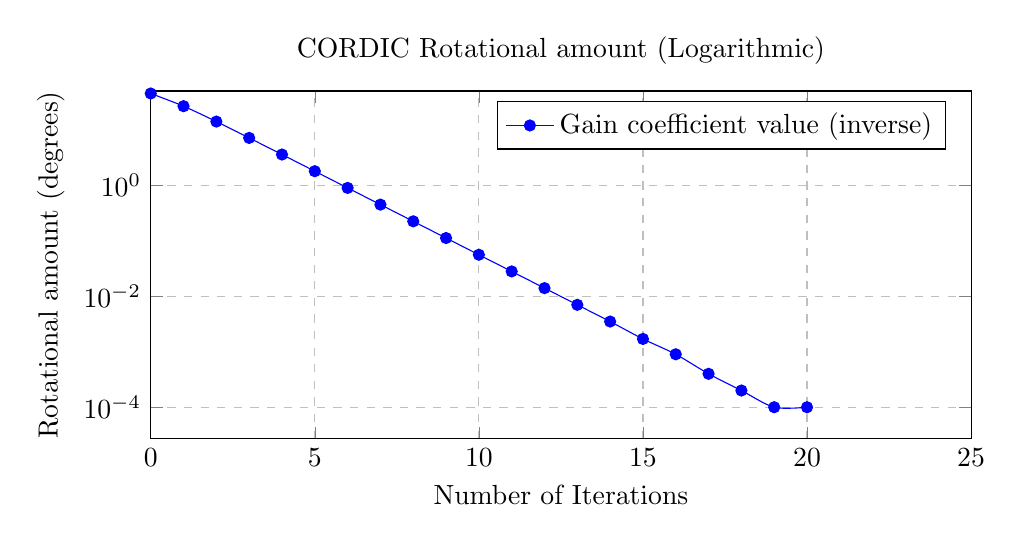
\begin{tikzpicture}

  \begin{axis}[    
  title={CORDIC Rotational amount (Logarithmic)},
      xlabel={Number of Iterations},
         ylabel={Rotational amount (degrees)},
         xmin=0,
         xmax=25,
         ymin=0,
         ymax=50,
         ymode=log,
         xtick={0, 5,..., 25},    
         ytick={},
         xmajorgrids=true,
		ymajorgrids=true,   
         legend pos=north east,    
         grid style={dashed,gray!50},    
         width=12cm, 
         height=6cm,    ]
          
\addplot[
color=blue,
mark=*,
smooth,
]
coordinates {
(0, 45)
(1, 26.565)
(2, 14.036)
(3, 7.125)
(4, 3.576)
(5, 1.790)
(6, 0.895)
(7, 0.4476)
(8, 0.2238)
(9, 0.1119)
(10, 0.0559)
(11, 0.0280)
(12, 0.0140)
(13, 0.0070)
(14, 0.0035)
(15, 0.0017)
(16, 0.0009)
(17, 0.0004)
(18, 0.0002)
(19, 0.0001)
(20, 0.0001)
};

\legend{Gain coefficient value (inverse)}

\end{axis}
\end{tikzpicture}
   \caption{Plot of CORDIC rotation per iteration (log)}
\end{center}
\end{figure}
\FloatBarrier

These results suggest that beyond approximately 8-10 levels of precision, there's not much room to gain in terms of approaching the true value of a given angle calculation. 

\subsection{Determination of precision}

To validate the theory of higher-iteration algorithms and their resultant precision, we implement the CORDIC algorithm in Vitis HLS and perform hardware simulations on a datapoint. Of course, the larger the piece of data is, the more deviation will be apparent in a final calculated value. For the test, we use the input cartesian vector
\begin{equation}
	\overline X = (325, 325)
\end{equation}
which, using traditional trigometry, converts to the polar form of
\begin{equation}
	\overline {X^*} = (r, \theta) = (459.619407771256, \pi / 4) = (459.619407771256, 0.785398163397448)
\end{equation}
where $\overline {X^*}$ is our "true value" we wish to calculate (or closely approach) using the CORDIC algorithm. Running the CORDIC using the datatype \codeword{FIXED_POINT} (refer to Listing \ref{datatypeHeader}), we determine the following results for magnitude and phase:

%% PLOT OF MAGNITUDE GOES HERE

\begin{figure}[h!]
\begin{center}
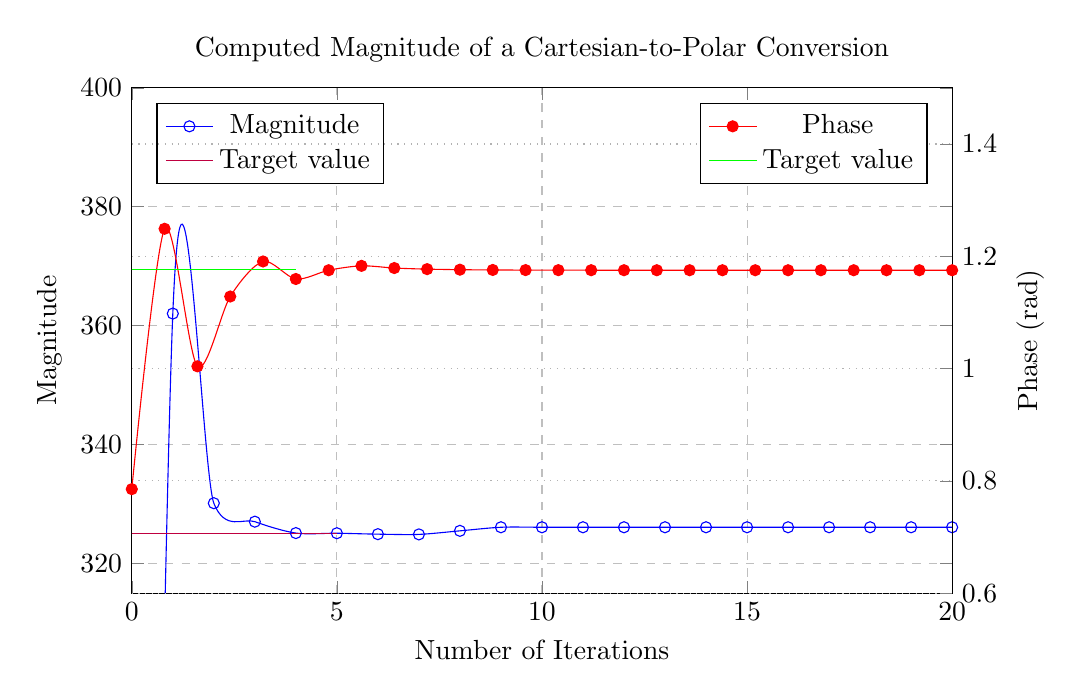
\begin{tikzpicture}

  \begin{axis}[    
  title={Computed Magnitude of a Cartesian-to-Polar Conversion},
      xlabel={Number of Iterations},
         ylabel={Magnitude},
         xmin=0,
         xmax=20,
         ymin=315,
         ymax=400,
         xtick={0, 5,..., 29},    
         ytick={},
         xmajorgrids=true,
		ymajorgrids=true,   
         legend pos=north west,    
         grid style={dashed,gray!50},    
         width=12cm, 
         height=8cm,    ]
          
\addplot[
color=blue,
mark=o,
smooth,
]
coordinates {
(0, 0.000000)
(1, 362.038666)
(2, 330.141785)
(3, 327.033875)
(4, 325.117310)
(5, 325.091827)
(6, 324.933197)
(7, 324.893524)
(8, 325.490875)
(9, 326.095673)
(10, 326.095032)
(11, 326.094879)
(12, 326.094849)
(13, 326.094849)
(14, 326.094849)
(15, 326.094849)
(16, 326.094849)
(17, 326.094849)
(18, 326.094849)
(19, 326.094849)
(20, 326.094849)
(21, 326.094849)
(22, 326.094849)
(23, 326.094849)
(24, 326.094849)
(25, 326.094849)
(26, 326.094849)
(27, 326.094849)
(28, 326.094849)
(29, 326.094849)
};

\addlegendentry{Magnitude}

\addplot[
color = purple,
mark=none,
smooth]
{325};

\addlegendentry{Target value}

\end{axis}
\begin{axis}[
         ylabel={Phase (rad)},
         xmin=0,
         xmax=25,
         axis x line = none,
         axis y line*=right,
         ymin=0.6,
         ymax=1.5,
         xtick={0, 5,..., 29},    
         ytick={},
         xmajorgrids=true,
		ymajorgrids=true,   
         legend pos=north east,    
         grid style={dotted,gray!60},    
         width=12cm, 
         height=8cm,    ]
         
         \addplot[
         color = red,
         mark = *,
         smooth]
         coordinates{
         (0, 0.785398)
(1, 1.249046)
(2, 1.004067)
(3, 1.128422)
(4, 1.190841)
(5, 1.159601)
(6, 1.175225)
(7, 1.183037)
(8, 1.179131)
(9, 1.177178)
(10, 1.176201)
(11, 1.175713)
(12, 1.175469)
(13, 1.175347)
(14, 1.175286)
(15, 1.175255)
(16, 1.175240)
(17, 1.175232)
(18, 1.175228)
(19, 1.175227)
(20, 1.175226)
(21, 1.175225)
(22, 1.175225)
(23, 1.175225)
(24, 1.175225)
(25, 1.175225)
(26, 1.175225)
(27, 1.175225)
(28, 1.175225)
(29, 1.175225)
         };
         
         \addlegendentry{Phase}
    \addplot[
color = green,
mark=none,
smooth]
{1.17600521};

\addlegendentry{Target value}
\end{axis}
\end{tikzpicture}
   \caption{Converted magnitude and phase of a cartesian vector}
\end{center}
\end{figure}
\FloatBarrier

We see that beyond 10 iterations, there is no significant improvement in the algorithm's computed result. Therefore, it is wise to avoid iterations beyond this amount. For the purposes of the accelerator, the number of iterations was fixed to 8.


\section{Optimization}

The algorithmic structure of the CORDIC is conducive to optimization. Unlike a FIR filter's convolutional structure, the CORDIC is a simple fixed-length iterative process that is immediately structured for optimization via parallelism.  Given that observation, we optimize the code structure using the precompiler directive \codeword{#pragma HLS PIPELINE} within the main rotation algorithm. This is shown below in Listing \ref{CORDICpipeline}.

		\begin{singlespace}
            \lstinputlisting[breaklines=true,
            label={CORDICpipeline},
            caption={Pipeline optimization},
            style=c-style,
            language=C++,
            firstnumber=136,
            linerange={136-139},
            ]{../source/CORDIC.cpp}
        \end{singlespace}


The pipelined algorithm allows parallel usage of hardware. This reduces latency significantly in the design, and increases the overall throughput of the processing chain. This is the only optimization performed to the CORDIC, which despite its simplicity, achieves a design latency as noted in Figure \ref{optimizedFIRutil}.















\end{document}